\ifx\bookloaded\undefined
\documentclass{article}
\ifx\pdftexversion\undefined
  \usepackage[dvips]{graphicx}
\else
  \usepackage[pdftex]{graphicx}
\fi
\newcommand{\be}{\begin{equation}}
\newcommand{\ee}{\end{equation}}
\newcommand{\rmmat}[1]{\hbox{\rm #1}}
\newcommand{\rmscr}[1]{{\hbox{\rm \scriptsize #1}}}
\newcommand{\comment}[1]{\relax}
\begin{document}
\fi

\section{Chapter 9} 
\begin{enumerate}
\item{\bf Lifetime}

Derive the lifetime of the $n=2, l=1, m=0$ state of hydrogen to emit a
photon and end up in the $n=1, l=0, m=0$ state.

{\bf Answer:}

The Einstein $A$-coefficient gives the rate of spontaneous emission
for a state
\begin{equation}
A_{21} = \frac{2h\nu^3}{c^2} B_{21} = \frac{32 \pi^3 \nu^3}{3 \hbar
  c^3} |{\bf d}_{if}|^2  = \frac{32 \pi^3 \nu^3}{3 \hbar
  c^3} e^2 a_0^2 \left |\frac{{\bf r}_{if}}{a_0} \right |^2 
\end{equation}
Let's calculate everything expect the matrix element to be sure of the
units.   We know that
\begin{equation}
h\nu = 2\pi \hbar \nu = \frac{e^2}{2 a_0} \left ( 1 - \frac{1}{2^2} \right ) = \frac{3
  e^2}{8 a_0}
\end{equation}
so we get
\begin{equation}
A_{21} = \frac{9 e^8}{128 \hbar^4 c^3 a_0}  \left |\frac{{\bf
    r}_{if}}{a_0} \right |^2  = \frac{9 \alpha^4}{128} \frac{c}{a_0} \left |\frac{{\bf
    r}_{if}}{a_0} \right |^2 = 1.13 \times 10^9 \rmmat{s}^{-1} \left |\frac{{\bf
    r}_{if}}{a_0} \right |^2
\end{equation}
where we used $\alpha=e^2/(\hbar c)$, so the units are clearly right!

The last step is to calculate the matrix element.  We will choose the
electron to initially be in the $m=0$ state so the $x$ and $y$
components of the dipole matrix element will be zero, so we are left with
\begin{eqnarray}
\frac{{\bf r}_{if}}{a_0} &=&  
\frac{2\pi}{a_0^5} \int_0^\infty r^2 dr \int_{-1}^1 d\mu \frac{1}{\sqrt{\pi}} e^{-r} (r\mu)
\frac{1}{4\sqrt{2\pi}} r e^{-r/2} \mu \\
&=& \frac{1}{2 \sqrt{2} a_0^5} \int_0^\infty dr  r^4 e^{-3r/2}
\int_{-1}^1 d\mu  \mu^2 = \frac{2^7\sqrt{2}}{3^5} = 0.745\\
\end{eqnarray}
The lifetime is
\begin{equation}
\frac{1}{A_{21}} = \left ( \frac{3}{2} \right )^8  \frac{a_0}{c}
\frac{1}{\alpha^4} =  \left ( \frac{3}{2} \right )^8  \frac{\hbar}{m_e
  c^2} \frac{1}{\alpha^5} = 1.58~\rmmat{ns}
\end{equation}
\item{\bf Hydrogen-Like Absorption}

How much energy does a photon need to ionize the following atoms by
removing a K-shell electron?  

Hydrogen, Helium, Carbon, Oxygen, Iron

Using the formula that I derived in class, draw an energy diagram that
shows the total cross section for one gram of gas as a function of
energy between 10eV and 10keV.   It would be great if you used the
initial expression in Eq. (72) for the dipole matrix element rather
than the final answer given by Eq. (73).

Consider that the mass fraction of the different atoms are hydrogen
(0.7), helium (0.27), carbon (0.008), oxygen (0.016) and iron (0.004).

{\bf Answer: }

Let's first get the units right like in the previous quesiton.   Using
equations (72) and (61) we get
\begin{equation}
\sigma_{bf} = \frac{2 p V m \omega}{3 c \hbar^3} 
\frac{256\pi}{V} \left ( \frac{Z}{a_0^2} \right )^5 
\left ( \frac{Z}{a_0^2} + q^2 \right )^{-6} e^2 q^2
\end{equation}
Let's relate $p=\hbar q$ to the energy of the photon, we have
\begin{equation}
E = \hbar \omega = \frac{p^2}{2 m} + E_I = \frac{p^2}{2 m} +
\frac{Z^2 \alpha^2}{2} 
 m c^2
\end{equation}
Let's define $x=E/E_I$ to get
\begin{equation}
\sigma_{bf} = \frac{256 \pi}{3 Z^2} \frac{1}{\alpha} \left (
\frac{\hbar}{m c} \right )^2 ( x - 1 )^{3/2} x^{-5} = \frac{32}{Z^2
  \alpha^3} \sigma_T ( x - 1 )^{3/2} x^{-5} 
\end{equation}
I know that $\sigma_T/m_p = 0.4~\rmmat{cm}^2 \rmmat{g}^{-1}$ so the
total cross section per gram of matertial is
\begin{equation}
\sigma_{bf,\rmscr{Total}} = \sum_i X_i \frac{\sigma_T}{m_p} 
\frac{32}{A_i Z_i^2
  \alpha^3} ( x_i - 1 )^{3/2} x_i^{-5} 
\end{equation}
where $X_i$ is the mass fraction of the species, $A_i$ is its atomic
weight, $Z_i$ is its atomic number and $x_i=E/(Z^2 13.6~\rmmat{eV})$.

{
\centering
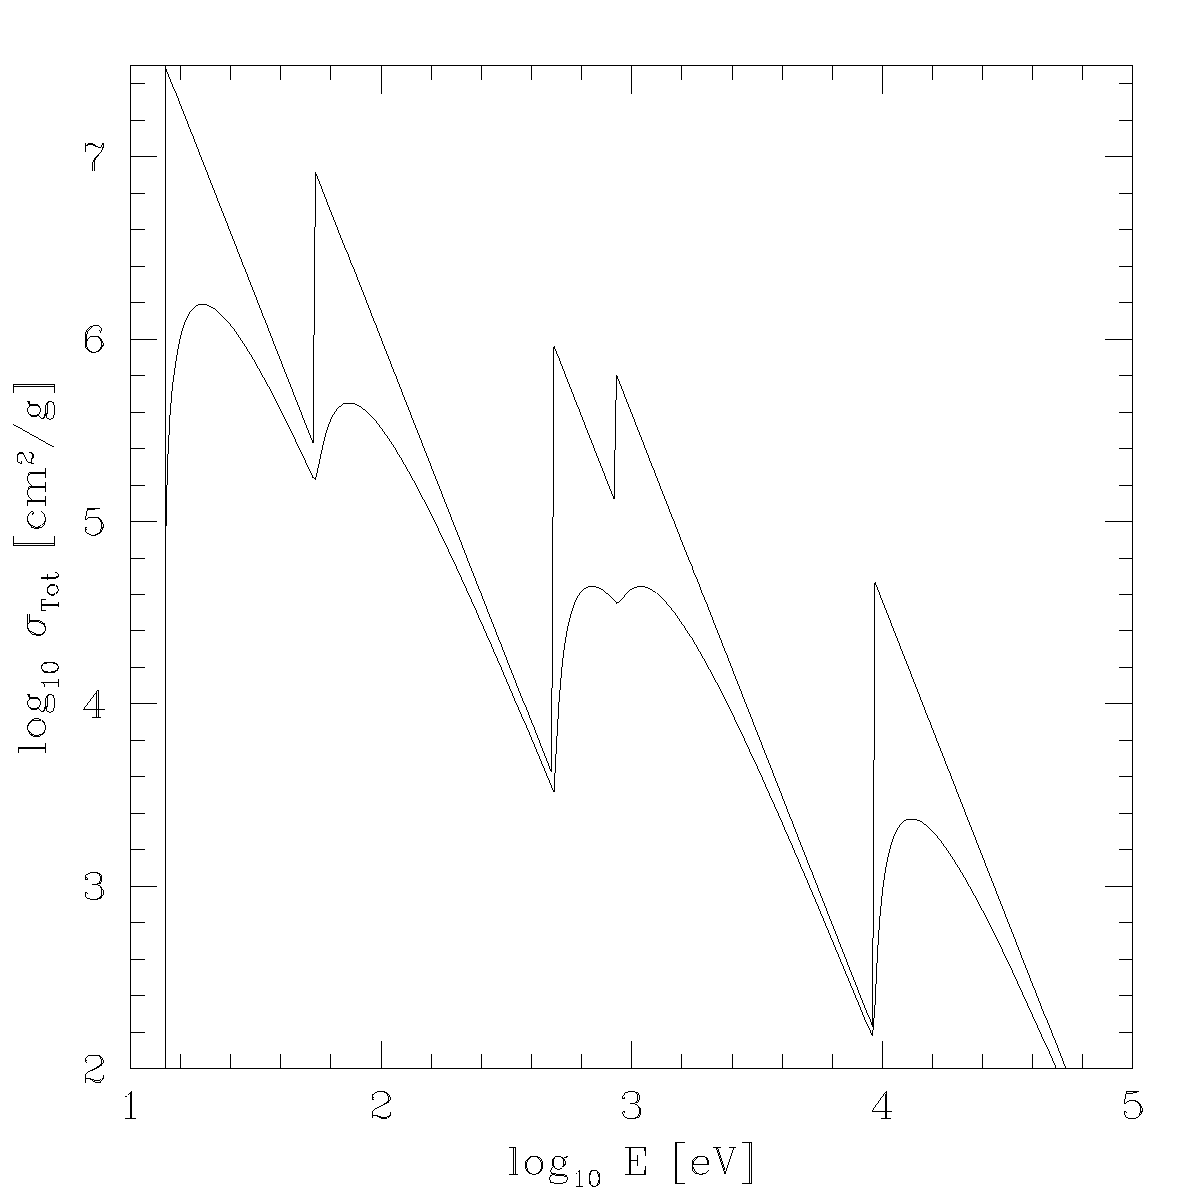
\includegraphics[width=0.9\textwidth]{week9cross} }
\end{enumerate}

\ifx\bookloaded\undefined
\end{document}
\end
\fi
